\documentclass[12pt,a4paper]{article}
\usepackage{amsmath,amssymb,mathtools}
\usepackage{geometry}
\geometry{margin=1in}
\usepackage{microtype}
\usepackage{caption}      % optional but recommended
\usepackage{subcaption} 
\usepackage{tikz}
\usetikzlibrary{arrows.meta}

\usepackage{enumitem}

\usepackage{fancyhdr}
\pagestyle{fancy}

\fancyhf{}

\fancyfoot[C]{\thepage}

	\fancyhead[L]{\textit{Two-by-two mapping charts}}
\fancyhead[R]{\textit{Exercises}}

% --- HEADER ---


\tikzset{
	>={Latex[length=2.6mm]},
	axis/.style={black, thin, ->},
	unitcircle/.style={black, very thin},
	pole/.style={red!70!black, fill=red!70!black},
	polemark/.style={red!70!black, thick},
	removable/.style={black, thick},
	essstar/.style={yellow!65!orange, star, star points=7, minimum size=6pt, draw=orange!80!black, fill=yellow!70!orange},
	lattice/.style={blue!70!black, fill=blue!70!black},
	note/.style={black!70, font=\scriptsize}
}
\usetikzlibrary{arrows.meta,shapes.geometric}

% --- colors and styles for the charts ---
\definecolor{PoleRed}{RGB}{214,49,56}
\definecolor{SimpleBlue}{RGB}{31,119,180}
\definecolor{Gold}{RGB}{247,183,51}

% styles
\definecolor{PoleRed}{RGB}{214,49,56}
\tikzset{
	>={Latex[length=3.4mm]},
	axis/.style={black, line width=1.0pt, ->},
	pole2/.style={PoleRed, line width=1.8pt},
	removable/.style={black, line width=1.6pt},
	leader/.style={black!70, line width=0.9pt},
	labelfunc/.style={font=\large},
	labeltext/.style={black!85, font=\normalsize},
	callout/.style={
		draw=black!40, fill=white, rounded corners=3pt,
		inner sep=5pt, outer sep=5pt,
		text=black, opacity=1, text opacity=1  % <- force visible text
	},
}



\title{Two-by-two mapping charts for $K_t(z)=\dfrac{e^{it}+z}{\,e^{it}-z\,}$}
\author{}
\date{}

\begin{document}
	\maketitle
	

	
	\paragraph{Description.}
	The Möbius kernel $K_t$ maps $\mathbb{D}$ conformally onto $\{w:\operatorname{Re}w>0\}$.
	In the $z$-plane, the level sets $\{\operatorname{Re}K_t=c\}$ (blue) and $\{\operatorname{Im}K_t=b\}$ (red)
	are two orthogonal pencils of circles, both tangent to $\partial\mathbb{D}$ at $\tau=e^{it}$.
	They correspond, respectively, to vertical and horizontal lines in the image half-plane.
	
	\bigskip
	
	% rotate domain charts by angle t (degrees)
	\def\tdeg{30}
	
	\tikzset{
		>={Latex[length=3mm]},
		boundary/.style={black, very thick},
		axis/.style={black, thin, ->},
		regrid/.style={blue!60!black, thick},
		imgrid/.style={red!70!black, thick}
	}
	
	% ---------- PANEL A: z-plane, Re K_t = const ----------
	\newcommand{\PanelZRe}{%
		\begin{tikzpicture}[scale=2.25]
			\begin{scope}[rotate=\tdeg]
				\draw[boundary] (0,0) circle (1);
				\draw[axis] (-1.15,0)--(1.2,0);
				\draw[axis] (0,-1.15)--(0,1.2);
				\fill (1,0) circle (0.03);
				\node[below left=2pt] at (1,0) {$\tau=e^{it}$};
				% Re K_t = c: centers (1/(1+c),0), radii 1/(1+c)
				\foreach \c in {0.3,1,3}{
					\pgfmathsetmacro{\xc}{1/(1+\c)}
					\pgfmathsetmacro{\rc}{1/(1+\c)}
					\draw[regrid] (\xc,0) circle (\rc);
				}
			\end{scope}
		\end{tikzpicture}
	}
	
	% ---------- PANEL B: w-plane, vertical lines ----------
	\newcommand{\PanelWRe}{%
		\begin{tikzpicture}[scale=2.25]
			\draw[axis] (-0.2,0)--(2.2,0) node[right] {$\operatorname{Re}w$};
			\draw[boundary] (0,-1.2)--(0,1.2);
			\node[left] at (0,1.2) {$\operatorname{Re}w=0$};
			\foreach \c in {0.3,1,3}{
				\draw[regrid] (\c,-1.2)--(\c,1.2);
			}
		\end{tikzpicture}
	}
	
	% ---------- PANEL C: z-plane, Im K_t = const ----------
	\newcommand{\PanelZIm}{%
		\begin{tikzpicture}[scale=2.25]
			\begin{scope}[rotate=\tdeg]
				\draw[boundary] (0,0) circle (1);
				\draw[axis] (-1.15,0)--(1.2,0);
				\draw[axis] (0,-1.15)--(0,1.2);
				\fill (1,0) circle (0.03);
				\node[below left=2pt] at (1,0) {$\tau=e^{it}$};
				% Im K_t = b: centers (1,1/b), radii |1/b|  (avoid b = 0)
				\foreach \b in {-2,-1,1,2}{
					\pgfmathsetmacro{\yc}{1/(\b)}
					\pgfmathsetmacro{\rb}{abs(\yc)}
					\draw[imgrid] (1,\yc) circle (\rb);
				}
			\end{scope}
		\end{tikzpicture}
	}
	
	% ---------- PANEL D: w-plane, horizontal lines ----------
	\newcommand{\PanelWIm}{%
		\begin{tikzpicture}[scale=2.25]
			\draw[axis] (-0.2,0)--(2.2,0) node[right] {$\operatorname{Re}w$};
			\draw[boundary] (0,-1.2)--(0,1.2);
			\node[left] at (0,1.2) {$\operatorname{Re}w=0$};
			\foreach \b in {-2,-1,1,2}{
				\draw[imgrid] (0,\b)--(2.1,\b);
			}
		\end{tikzpicture}
	}
	
	% ==================== ROW 1: verticals ====================
	\begin{center}
		\begin{minipage}[t]{0.49\textwidth}\centering
			\textbf{Domain: $z$-plane (vertical family)}\\[0.3em]
			\PanelZRe
		\end{minipage}\hfill
		\begin{minipage}[t]{0.49\textwidth}\centering
			\textbf{Image: $w$-plane (vertical lines)}\\[0.3em]
			\PanelWRe
		\end{minipage}
	\end{center}
	
	\vspace{1.1em}
	\begin{center}\small
		Blue circles $\{\operatorname{Re}K_t=c\}$ in the domain $\longleftrightarrow$ blue vertical lines $\{\operatorname{Re}w=c\}$ in the image.
	\end{center}
	
	% ==================== ROW 2: horizontals ====================
	\vspace{1.6em}
	\begin{center}
		\begin{minipage}[t]{0.49\textwidth}\centering
			\textbf{Domain: $z$-plane (horizontal family)}\\[0.3em]
			\PanelZIm
		\end{minipage}\hfill
		\begin{minipage}[t]{0.49\textwidth}\centering
			\textbf{Image: $w$-plane (horizontal lines)}\\[0.3em]
			\PanelWIm
		\end{minipage}
	\end{center}
	
	\vspace{1.1em}
	\begin{center}\small
		Red circles $\{\operatorname{Im}K_t=b\}$ in the domain $\longleftrightarrow$ red horizontal lines $\{\operatorname{Im}w=b\}$ in the image.
	\end{center}
	
	

	
% ========================= FIGURE: singularity charts =========================
\begin{figure}[t]
	\centering
	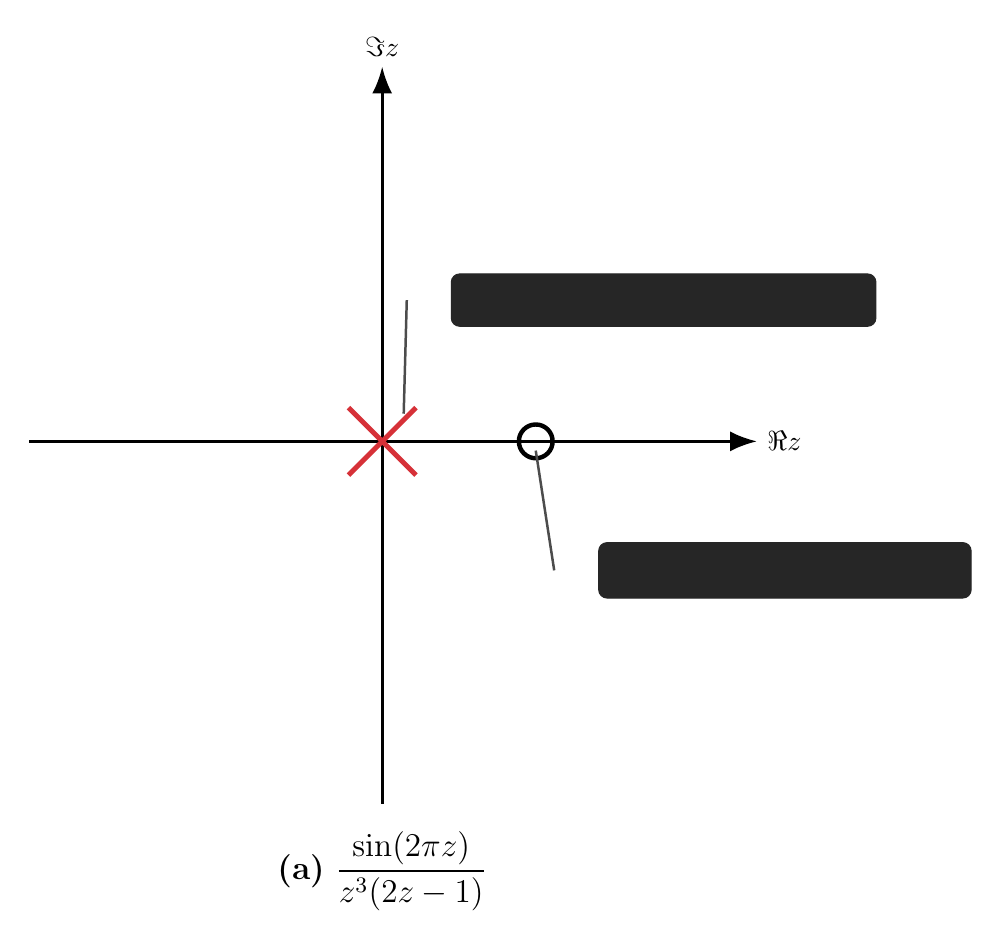
\begin{tikzpicture}[scale=3.9]
		\draw[axis] (-1.15,0)--(1.22,0) node[right] {$\Re z$};
		\draw[axis] (0,-1.18)--(0,1.22) node[above] {$\Im z$};
		
		% pole (order 2) at 0
		\draw[pole2] (-0.11,-0.11)--(0.11,0.11);
		\draw[pole2] (-0.11,0.11)--(0.11,-0.11);
		
		% removable at 1/2
		\draw[removable] (0.5,0) circle (0.055);
		
		% callouts (plain white boxes, black text)
		\node[callout, labeltext, anchor=west] (A1) at (0.18,0.46)
		{pole of order $2$ at $0$; residue $-4\pi$};
		\draw[leader] ([xshift=-0.10cm]A1.west) -- (0.07,0.09);
		
		\node[callout, labeltext, anchor=west] (A2) at (0.66,-0.42)
		{removable at $1/2$ (residue $0$)};
		\draw[leader] ([xshift=-0.10cm]A2.west) -- (0.50,-0.03);
		
		\node[labelfunc] at (0,-1.40) {\textbf{(a)} $\displaystyle \frac{\sin(2\pi z)}{z^{3}(2z-1)}$};
	\end{tikzpicture}
	
	\caption{\textbf{Panel (a).} The function $\sin(2\pi z)/(z^{3}(2z-1))$ has a double pole at $z=0$ with residue $-4\pi$ and a removable singularity at $z=\tfrac12$ (residue $0$).}
\end{figure}

	
	\clearpage
	
	\section*{Conformal maps: an overview catalogue (no details)}
	
	\begin{enumerate}
		\item \textbf{Cayley (disk $\leftrightarrow$ right half-plane).}\\[2pt]
		\[
		\boxed{\,w=\frac{1+z}{1-z}\,}\qquad\text{inverse:}\quad z=\frac{w-1}{w+1}.
		\]
		
		\item \textbf{Half-plane $\to$ half-plane (three-point normalization).}\\[2pt]
		\[
		\boxed{\,w=\frac{(z-a)(c-b)}{(z-b)(c-a)}\,}.
		\]
		
		\item \textbf{Disk automorphisms.}\\[2pt]
		\[
		\boxed{\,\phi_{a,\theta}(z)=e^{i\theta}\frac{z-a}{1-\bar a z}\,},\qquad |a|<1.
		\]
		
		\item \textbf{Strip $|\Im z|<h/2$ $\to$ right half-plane.}\\[2pt]
		\[
		\boxed{\,w=\exp\!\left(\frac{\pi z}{h}\right)\,}.
		\]
		
		\item \textbf{Strip $|\Im z|<h/2$ $\to$ unit disk.}\\[2pt]
		\[
		\boxed{\,\zeta=\frac{e^{\pi z/h}-1}{\,e^{\pi z/h}+1\,}\,}.
		\]
		
		\item \textbf{Strip $\to$ strip (height scaling).}\\[2pt]
		\[
		\boxed{\,z\mapsto \frac{h_2}{h_1}\,z\,}.
		\]
		
		\item \textbf{Band $a<\Im z<b$ $\to$ centered strip.}\\[2pt]
		\[
		\boxed{\,z\mapsto \frac{\pi}{b-a}\!\left(z-i\frac{a+b}{2}\right)\,}.
		\]
		
		\item \textbf{Sector $\{0<\arg z<\alpha\}$ $\to$ upper half-plane.}\\[2pt]
		\[
		\boxed{\,w=z^{\pi/\alpha}\,}\ \ \text{(principal branch)}.
		\]
		
		\item \textbf{Wedge $\to$ disk.}\\[2pt]
		Compose item (8) with Cayley (item 1).
		
		\item \textbf{Upper half-plane $\to$ disk (prescribed triple).}\\[2pt]
		\[
		\boxed{\,\Phi(z)=\frac{(z-a)}{(z-\bar a)}\cdot \frac{(b-\bar a)}{(b-a)}\,}.
		\]
		
		\item \textbf{Annulus $r<|z|<1$ $\leftrightarrow$ strip.}\\[2pt]
		\[
		\boxed{\,w=\log z\,}\quad\text{maps to }\ \log r<\Re w<0.
		\]
		
		\item \textbf{Annulus $\to$ disk.}\\[2pt]
		Use $w=\log z$ then item (5).
		
		\item \textbf{Half-plane minus disk $\to$ annulus.}\\[2pt]
		\[
		\boxed{\,\zeta=\frac{z-\alpha}{z+\alpha}\,},\qquad \alpha^{2}=a^{2}-b^{2}.
		\]
		
		\item \textbf{Disk with off-center hole $\to$ annulus.}\\[2pt]
		Center via $\phi_a$ (item 3), then items (11)–(12).
		
		\item \textbf{Punctured plane $\leftrightarrow$ cylinder.}\\[2pt]
		\[
		\boxed{\,w=\log z\,}\quad(\text{period }2\pi i).
		\]
		
		\item \textbf{Strip $\to$ punctured plane.}\\[2pt]
		\[
		\boxed{\,z\mapsto e^{z}\,}.
		\]
		
		\item \textbf{Ray-slit plane $\mathbb C\setminus[0,\infty)$ $\to$ half-plane.}\\[2pt]
		\[
		\boxed{\,w=\sqrt{z}\,}\ \ \text{(choose branch)}.
		\]
		
		\item \textbf{Segment-slit plane $\mathbb C\setminus[a,b]$ $\to$ half-plane.}\\[2pt]
		\[
		\boxed{\,w=\sqrt{\frac{z-a}{\,z-b\,}}\,}.
		\]
		
		\item \textbf{Exterior of $[-1,1]$ $\leftrightarrow$ exterior unit circle (Joukowski).}\\[2pt]
		\[
		\boxed{\,w=z+\frac{1}{z}\,},\qquad
		z=\frac{w\pm\sqrt{w^{2}-4}}{2}.
		\]
		
		\item \textbf{Exterior of ellipse $\leftrightarrow$ exterior unit circle.}\\[2pt]
		\[
		\boxed{\,w=\tfrac12\!\left(c z+\frac{1}{c z}\right)\,}\quad(\text{$c$ from axes}).
		\]
		
		\item \textbf{Right half-plane $\to$ vertical strip.}\\[2pt]
		\[
		\boxed{\,z\mapsto \frac{1}{\pi}\log\frac{z-1}{\,z+1\,}\,}.
		\]
		
		\item \textbf{Upper half-plane $\to$ rectangle (SC/elliptic).}\\[2pt]
		\[
		\boxed{\,\zeta=\int^z \frac{dt}{\sqrt{(t-a)(t-b)(t-c)(t-d)}}\,}.
		\]
		
		\item \textbf{Rectangle $\to$ disk (Jacobi sn).}\\[2pt]
		\[
		\boxed{\,\zeta=\operatorname{sn}\!\left(\frac{K(k)}{L}\,z;\,k\right)\,}.
		\]
		
		\item \textbf{Half-disk $\leftrightarrow$ half-plane.}\\[2pt]
		Restriction of Cayley (item 1) and inverse.
		
		\item \textbf{Lens (intersection of two disks) $\to$ disk.}\\[2pt]
		Möbius normalizes the circles; then a power map; then Cayley.
		
		\item \textbf{Half-strip $\{x>0,\ 0<\Im z<h\}$ $\to$ half-disk.}\\[2pt]
		\[
		\boxed{\,\exp(\pi z/h)\,}\ \ \text{then power, then Cayley}.
		\]
		
		\item \textbf{Polygon $\to$ half-plane (Schwarz--Christoffel).}\\[2pt]
		\[
		\boxed{\,\Phi'(z)=C\prod_k (z-z_k)^{\alpha_k-1}\,},\qquad \sum\alpha_k=2.
		\]
		
		\item \textbf{Upper half-plane $\to$ slit half-plane.}\\[2pt]
		\[
		\boxed{\,w=z+\frac{1}{z}\,}\ \ \text{then a real Möbius adjustment}.
		\]
		
		\item \textbf{Disk $\to$ disk with boundary arc removed.}\\[2pt]
		Automorphism to put endpoints at $\pm1$, then boundary power $z^\lambda$.
		
		\item \textbf{Finite Blaschke product (disk $\to$ disk, degree $n$).}\\[2pt]
		\[
		\boxed{\,B(z)=e^{i\theta}\prod_{k=1}^n \frac{z-a_k}{\,1-\bar a_k z\,}\,}.
		\]
	\end{enumerate}
	
	
	
	
	\section*{1.\ Cayley transform: $\mathbb D \leftrightarrow$ right half-plane}
	
	\paragraph{Map and inverse.}\mbox{}\\[2pt]
	\[
	w=\frac{1+z}{\,1-z\,}
	\quad\text{maps}\quad
	\mathbb D=\{|z|<1\}\ \text{onto}\ \{\,\Re w>0\,\},
	\qquad
	z=\frac{w-1}{\,w+1\,}
	\]
	is the inverse.
	
	\medskip
	
	\paragraph{Why $\Re w>0$.}\mbox{}\\[2pt]
	Compute
	\[
	\Re\!\left(\frac{1+z}{\,1-z\,}\right)
	=\frac{\,1-|z|^{2}\,}{\,|1-z|^{2}\,}.
	\]
	Thus $\Re w>0$ for $|z|<1$, and $\Re w=0$ for $|z|=1$ (except $z=1$, which maps to $w=\infty$).
	Therefore
	\[
	|z|<1\ \Longleftrightarrow\ \Re w>0,
	\qquad
	|z|=1\ \Longleftrightarrow\ \Re w=0 .
	\]
	
	\medskip
	
	\paragraph{Boundary correspondence.}\mbox{}\\[2pt]
	$z=0\mapsto w=1$,
	\quad
	$z\to1^{-}\mapsto w\to+\infty$,
	\quad
	and $\partial\mathbb D\setminus\{1\}$ maps to the line $\Re w=0$.\\[2pt]
	Circles/lines orthogonal to $\partial\mathbb D$ map to \emph{vertical} lines in the $w$–plane.
	
	
	\section*{Cayley transform: \(\mathbb D \leftrightarrow\) right half-plane}
	
	Consider the Cayley transform
	\[
	w = \phi(z) := \frac{1+z}{1-z}, 
	\qquad
	z = \phi^{-1}(w) = \frac{w-1}{w+1}.
	\]
	Then
	\[
	\Re w 
	= \Re\!\left(\frac{1+z}{1-z}\right)
	= \frac{1-|z|^2}{|1-z|^2}.
	\]
	Hence
	\[
	|z| < 1 \iff \Re w > 0,
	\qquad
	|z| = 1,\; z\neq 1 \iff \Re w = 0.
	\]
	Thus the Cayley transform maps the unit disc
	\(\mathbb D = \{\,|z|<1\,\}\) biholomorphically onto the right
	half-plane \(\{\,w : \Re w>0\,\}\), and the unit circle
	\(\partial\mathbb D \setminus \{1\}\) onto the imaginary axis.
	
	\subsubsection*{Images of lines and circles}
	
	Because \(\phi\) is a Möbius transformation, it maps generalized circles
	(lines or circles) in the \(z\)-plane to generalized circles in the
	\(w\)-plane. In particular:
	
	\begin{itemize}
		\item For \(0<r<1\), the circle \(|z|=r\) is orthogonal to the unit
		circle and is mapped to a vertical line in the right half-plane.
		A direct computation gives
		\[
		|z| = r 
		\quad\Longleftrightarrow\quad
		\Re w = \frac{1+r^2}{1-r^2} > 0.
		\]
		\item Radii \(z = t e^{i\theta}\), \(0\le t<1\), become circular arcs
		in the right half-plane, orthogonal to the boundary
		line \(\Re w=0\).
		\item Curves tangent to the unit circle at \(z=1\) are mapped to
		horizontal lines in the \(w\)-plane (parallel to the boundary).
	\end{itemize}
	
	\subsubsection*{Mapping charts}
	
	Figure~\ref{fig:cayley-z-grid} shows a polar grid inside the unit disc:
	several concentric circles and radii. In
	Figure~\ref{fig:cayley-w-grid} we see its image under the Cayley
	transform: concentric circles become vertical lines, radii become
	circular arcs, and the unit circle maps to the imaginary axis.
	
	\begin{figure}[ht]
		\centering
		
\includegraphics[width=0.6\textwidth]{.figs/cayley_z_grid.png}
		\caption{Grid in the unit disc (z-plane): unit circle, concentric
			circles, and radii.}
		\label{fig:cayley-z-grid}
	\end{figure}
	
	\begin{figure}[ht]
		\centering
		
\includegraphics[width=0.7\textwidth]{.figs/cayley_w_grid.png}
		\caption{Image of the disc under the Cayley transform in the
			\(w\)-plane: the unit circle becomes the imaginary axis, concentric
			circles become vertical lines, and radii become circular arcs
			orthogonal to the boundary.}
		\label{fig:cayley-w-grid}
	\end{figure}
	
	\subsubsection*{Vertical and horizontal lines}
	
	To visualise more explicitly how vertical and horizontal lines in the
	right half-plane look in the disc, consider the inverse Cayley transform
	\[
	z = \phi^{-1}(w) = \frac{w-1}{w+1}.
	\]
	
	\paragraph{Vertical lines.}
	Fix \(c>0\) and consider the vertical line
	\[
	L_c := \{\, w = c + it : t\in\mathbb R \,\}.
	\]
	Its preimage \(\phi^{-1}(L_c)\) is a circle inside the unit disc,
	orthogonal to \(\partial\mathbb D\). In particular, every vertical line
	\(\Re w = c\) intersects the boundary \(\Re w=0\) at right angles, and
	its preimage is a circle intersecting \(|z|=1\) at right angles.
	
	\paragraph{Horizontal lines.}
	Fix \(d\in\mathbb R\) and consider the horizontal line
	\[
	H_d := \{\, w = s + i d : s>0 \,\}.
	\]
	Its preimage \(\phi^{-1}(H_d)\) is a circle tangent to the unit circle
	at the point \(z=1\). Thus horizontal lines in the half-plane correspond
	to circles in the disc that ``aim at'' the boundary point mapped to
	infinity.
	
	\begin{figure}[ht]
		\centering
		
\includegraphics[width=0.7\textwidth]{.figs/cayley_lines_w.png}
		\caption{Families of vertical (solid) and horizontal (dashed) lines in
			the \(w\)-plane. The imaginary axis \(\Re w=0\) is the boundary of
			the image of the disc.}
		\label{fig:cayley-lines-w}
	\end{figure}
	
	\begin{figure}[ht]
		\centering
		
\includegraphics[width=0.6\textwidth]{.figs/cayley_lines_z.png}
		\caption{Preimages in the \(z\)-plane of the vertical and horizontal
			lines from Figure~\ref{fig:cayley-lines-w}. Vertical lines become
			circles orthogonal to the unit circle, while horizontal lines become
			circles tangent to \(\partial\mathbb D\) at \(z=1\).}
		\label{fig:cayley-lines-z}
	\end{figure}
	
	\subsubsection*{Vertical and horizontal chords in the disc}
	
	Besides the polar grid, it is instructive to see what happens to
	straight chords of the unit disc. Consider the vertical and horizontal
	segments
	\[
	\{ z = a + i y : a^2 + y^2 < 1 \}, \qquad
	\{ z = x + i b : x^2 + b^2 < 1 \},
	\]
	for fixed real numbers \(a,b\) with \(|a|,|b|<1\). These are vertical
	and horizontal lines in the \(z\)-plane, truncated to lie inside the
	disc.
	
	Under the Cayley transform
	\[
	w = \phi(z) = \frac{1+z}{1-z},
	\]
	each such chord is mapped to a generalized circle in the \(w\)-plane.
	In particular, the real axis segment
	\((-1,1)\subset\mathbb R\) (the chord \(\Im z=0\)) is mapped onto the
	positive real axis in the half-plane. Other vertical and horizontal
	chords are mapped to curved arcs lying entirely in the region
	\(\Re w>0\).
	
	\begin{figure}[ht]
		\centering
		
\includegraphics[width=0.6\textwidth]{.figs/cayley_z_chords.png}
		\caption{Vertical (solid) and horizontal (dashed) chords inside the
			unit disc.}
		\label{fig:cayley-z-chords}
	\end{figure}
	
	\begin{figure}[ht]
		\centering
		
\includegraphics[width=0.7\textwidth]{.figs/cayley_w_chords.png}
		\caption{Images of the chords from
			Figure~\ref{fig:cayley-z-chords} under the Cayley transform. Each
			chord becomes a generalized circle lying in the right half-plane;
			the real axis segment maps to the positive real axis.}
		\label{fig:cayley-w-chords}
	\end{figure}
	
	Fix real numbers $a,b$ with $|a|,|b|<1$. Consider the vertical and
	horizontal chords inside the unit disc
	\[
	\{ z = a + i y : a^2 + y^2 < 1 \}, \qquad
	\{ z = x + i b : x^2 + b^2 < 1 \}.
	\]
	These are the intersections of the vertical line $\Re z = a$ and the
	horizontal line $\Im z = b$ with the unit disc $|z|<1$.
	
	\bigskip\hrule\bigskip
	
	\section*{2.\ Three-point Möbius normalization: half-plane $\leftrightarrow$ half-plane}
	
	\paragraph{Cross-ratio map to the real axis.}\mbox{}\\[2pt]
	Let $L$ be a line or circle, and choose three distinct points $a,b,c\in L$. Define
	\[
	\Phi(z)=\frac{(z-a)(c-b)}{(z-b)(c-a)}.
	\]
	Then $\Phi(L)\subset\mathbb R\cup\{\infty\}$, with
	\[
	\Phi(a)=0,\qquad \Phi(b)=\infty,\qquad \Phi(c)=1,
	\]
	and the two sides of $L$ map to the half-planes $\Im\Phi(z)\gtrless 0$.
	
	
	\section*{Three-point M\"obius normalization: half-plane $\leftrightarrow$ half-plane}
	
	\subsubsection*{Cross-ratio map to the real axis}
	
	Let $L$ be a line or circle in the extended complex plane $\widehat{\mathbb C}$,
	and choose three distinct points $a,b,c\in L$. Define
	\[
	\Phi(z)
	= \frac{(z-a)(c-b)}{(z-b)(c-a)}.
	\]
	This is a M\"obius transformation with
	\[
	\Phi(a) = 0,\qquad
	\Phi(b) = \infty,\qquad
	\Phi(c) = 1.
	\]
	Moreover, one has
	\[
	\Phi(L) \subset \mathbb R \cup \{\infty\},
	\]
	so $L$ is mapped onto the real axis (possibly passing through $\infty$),
	and the two sides of $L$ are mapped to the two open half-planes
	$\Im \Phi(z) > 0$ and $\Im \Phi(z) < 0$.
	
	In other words, by fixing three marked points $a,b,c$ on $L$, the
	cross-ratio map $\Phi$ \emph{normalizes} the configuration so that these
	points become $0,\infty,1$ and $L$ itself becomes the real line.
	
	\subsubsection*{Example: a circle mapped to the real axis}
	
	As a concrete example, let $L$ be the unit circle
	\[
	L = \{ z\in\mathbb C : |z|=1 \},
	\]
	and choose three distinct points on $L$:
	\[
	a = 1,\qquad b=-1,\qquad c=i.
	\]
	Then the associated map
	\[
	\Phi(z) = \frac{(z-a)(c-b)}{(z-b)(c-a)}
	\]
	sends $L$ onto the real axis, with
	\[
	\Phi(a)=0,\qquad \Phi(b)=\infty,\qquad \Phi(c)=1.
	\]
	For $z$ not on $L$, the sign of $\Im \Phi(z)$ indicates on which side of
	the circle $L$ the point $z$ lies. One side of $L$ (for instance, the
	interior) is mapped to the upper half-plane $\Im w>0$, while the other
	side (the exterior) is mapped to the lower half-plane $\Im w<0$.
	
	Figure~\ref{fig:crossratio-z-plane} illustrates this: we show the circle
	$L$, the points $a,b,c$, and a cloud of sample points in the plane,
	distinguished according to the sign of $\Im\Phi(z)$. In
	Figure~\ref{fig:crossratio-w-plane}, we see their images under $\Phi$,
	which lie strictly above or below the real axis.
	
	\begin{figure}[ht]
		\centering
		
\includegraphics[width=0.6\textwidth]{.figs/crossratio_z_plane.png}
		\caption{The unit circle $L$ (example of a generalized line) with
			three marked points $a,b,c\in L$ and sample points on its two sides.
			The two sides are distinguished according to the sign of
			$\Im\Phi(z)$, which will become the upper and lower half-planes in
			the $w$-plane.}
		\label{fig:crossratio-z-plane}
	\end{figure}
	
	\begin{figure}[ht]
		\centering
		
\includegraphics[width=0.7\textwidth]{.figs/crossratio_w_plane.png}
		\caption{Image of the configuration under the cross-ratio map
			$\Phi$. The circle $L$ is sent to the real axis, with
			$\Phi(a)=0$, $\Phi(b)=\infty$, $\Phi(c)=1$. Points on one side of
			$L$ land in the upper half-plane $\Im w>0$, and points on the other
			side land in the lower half-plane $\Im w<0$.}
		\label{fig:crossratio-w-plane}
	\end{figure}
	
	\subsubsection*{Example: a line mapped to the real axis}
	
	Now let $L$ be a straight line instead of a circle. Take, for instance,
	the imaginary axis
	\[
	L = \{ z = i y : y\in\mathbb R\},
	\]
	and choose three distinct points on $L$:
	\[
	a = i,\qquad b=-i,\qquad c=0.
	\]
	The corresponding cross-ratio map
	\[
	\Phi(z)
	= \frac{(z-a)(c-b)}{(z-b)(c-a)}
	\]
	again satisfies
	\[
	\Phi(a)=0,\qquad \Phi(b)=\infty,\qquad \Phi(c)=1,
	\]
	and sends the whole line $L$ onto the real axis
	$\mathbb R\cup\{\infty\}$. As before, the two sides of $L$ are mapped
	onto the upper and lower half-planes:
	\[
	\text{one side of } L \;\longmapsto\; \{ w : \Im w > 0\},\qquad
	\text{the other side} \;\longmapsto\; \{ w : \Im w < 0\}.
	\]
	
	Figure~\ref{fig:crossratio-line-z-plane} shows the line $L$ and some
	sample points on each side, distinguished by the sign of $\Im \Phi(z)$.
	Figure~\ref{fig:crossratio-line-w-plane} illustrates their images under
	$\Phi$: the line becomes the real axis, with $\Phi(a)=0$ and
	$\Phi(c)=1$, and the two sides become the upper and lower half-planes.
	
	\begin{figure}[ht]
		\centering
		
\includegraphics[width=0.65\textwidth]{.figs/crossratio_line_z_plane.png}
		\caption{The line $L$ (the imaginary axis) with marked points
			$a=i$, $b=-i$, $c=0$. Sample points on its two sides are labelled
			according to the sign of $\Im\Phi(z)$.}
		\label{fig:crossratio-line-z-plane}
	\end{figure}
	
	\begin{figure}[ht]
		\centering
		
\includegraphics[width=0.7\textwidth]{.figs/crossratio_line_w_plane.png}
		\caption{Image of the configuration under $\Phi$. The line $L$ is
			mapped to the real axis, with $\Phi(a)=0$, $\Phi(b)=\infty$,
			$\Phi(c)=1$. One side of $L$ maps to the upper half-plane
			$\Im w>0$, the other side to the lower half-plane $\Im w<0$.}
		\label{fig:crossratio-line-w-plane}
	\end{figure}
	
	\medskip
	
	\clearpage
	
\subsubsection*{Half-plane to half-plane via three boundary points}

Let $H_1,H_2$ be half-planes with boundary arcs $L_1,L_2$.
Choose boundary triples
\[
a,b,c \in L_1, \qquad A,B,C \in L_2
\]
in the same cyclic order as seen from the chosen sides of $H_1,H_2$.

First send $L_1$ to the real axis by the cross-ratio map
\[
\Phi(z) := \frac{(z-a)(c-b)}{(z-b)(c-a)}.
\]
Then $\Phi(a)=0$, $\Phi(b)=\infty$, $\Phi(c)=1$, and the two sides of
$L_1$ correspond to the half-planes $\Im\Phi(z)\gtrless 0$.

Next send $L_2$ to the real axis by
\[
\Psi(w) := \frac{(w-A)(C-B)}{(w-B)(C-A)},
\]
so that $\Psi(A)=0$, $\Psi(B)=\infty$, $\Psi(C)=1$.

The desired map $T : H_1 \to H_2$ is given by
\[
\Psi\bigl(T(z)\bigr) = \Phi(z),
\qquad\text{i.e.}\qquad
T(z) = \Psi^{-1}(\Phi(z)).
\]
Solving for $\Psi^{-1}$ yields the explicit formula
\[
T(z)
= \frac{A(C-B) - \Phi(z)\, B(C-A)}{(C-B) - \Phi(z)\,(C-A)},
\qquad
\Phi(z) = \frac{(z-a)(c-b)}{(z-b)(c-a)}.
\]
Then
\[
T(a)=A,\qquad T(b)=B,\qquad T(c)=C,
\]
and $T$ maps the chosen side of $H_1$ biholomorphically onto the chosen
side of $H_2$. If the orientation of the half-plane is reversed, one may
replace $\Phi$ by $-\Phi$ or interchange two of the boundary points to
flip the side.

\subsubsection*{Example: upper half-plane to right half-plane}

A particularly simple instance is obtained by taking
\[
T(z) = -i z.
\]
Then
\[
\Re T(z) = \Re(-iz) = \Im z,
\]
so
\[
\Im z > 0 \quad\Longleftrightarrow\quad \Re T(z) > 0.
\]
Thus $T$ maps the upper half-plane
\[
H_1 = \{ z : \Im z > 0 \}
\]
bijectively onto the right half-plane
\[
H_2 = \{ w : \Re w > 0 \},
\]
sending the boundary line $L_1 = \mathbb R$ to the boundary line
$L_2 = i\mathbb R$.

Figures~\ref{fig:hp-to-hp-z-plane-fixed} and
\ref{fig:hp-to-hp-w-plane-fixed} illustrate this example.

\begin{figure}[ht]
	\centering
	
\includegraphics[width=0.6\textwidth]{.figs/hp_to_hp_z_plane_fixed.png}
	\caption{Source half-plane $H_1 = \{\Im z>0\}$ with boundary
		$L_1=\mathbb R$ and a grid of sample points.}
	\label{fig:hp-to-hp-z-plane-fixed}
\end{figure}

\begin{figure}[ht]
	\centering
	
\includegraphics[width=0.7\textwidth]{.figs/hp_to_hp_w_plane_fixed.png}
	\caption{Image under $T(z)=-iz$: the upper half-plane is mapped to the
		right half-plane $H_2 = \{\Re w>0\}$, and the real axis is mapped to
		the imaginary axis $L_2=i\mathbb R$. All sample points lie strictly
		to the right of the boundary line.}
	\label{fig:hp-to-hp-w-plane-fixed}
\end{figure}

\medskip
\noindent
The above example is the simplest possible case of a half-plane to
half-plane mapping, since $T(z)=-iz$ is just a rotation by $-\pi/2$.
However, every biholomorphic map between half-planes can be obtained from
the general three–boundary–points construction described earlier.  In
particular, if $a,b,c$ are three distinct points on the boundary line
$L_1=\mathbb R$, and $A,B,C$ are three distinct points on the boundary
line $L_2=i\mathbb R$ in the same cyclic order, then the unique M\"obius
map satisfying
\[
T(a)=A,\qquad T(b)=B,\qquad T(c)=C
\]
is given explicitly by
\[
T(z)
= \frac{A(C-B) - \Phi(z)\, B(C-A)}{(C-B) - \Phi(z)\,(C-A)},
\qquad
\Phi(z) = \frac{(z-a)(c-b)}{(z-b)(c-a)}.
\]
This expression reduces to $T(z)=-iz$ precisely when the triples
$(a,b,c)$ and $(A,B,C)$ are chosen so that the cross-ratios coincide and
the real axis is mapped to the imaginary axis by a pure rotation.
Thus the simple rotation $T(z)=-iz$ is not an isolated coincidence, but
a special case of the general boundary-normalization principle.


\subsubsection*{Non–trivial example: half-plane to half-plane via three boundary points}

We now give a non-trivial instance of the general construction.  
Take three distinct boundary points on the real axis
\[
a=-2,\qquad b=1,\qquad c=4,
\]
and three distinct boundary points on the imaginary axis
\[
A=-i,\qquad B=0,\qquad C=2i,
\]
listed in the same cyclic order (bottom $\to$ top).

The cross-ratio map sending $a,b,c$ to $0,\infty,1$ is
\[
\Phi(z)
= \frac{(z-a)(c-b)}{(z-b)(c-a)}
= \frac{(z+2)(3)}{(z-1)(6)}.
\]

The inverse map sending $0,\infty,1$ back to $A,B,C$ is
\[
\Psi^{-1}(\xi)
= \frac{A(C-B) - \xi\,B(C-A)}{(C-B) - \xi\,(C-A)}.
\]

Hence the desired half-plane map is
\[
T(z) = \Psi^{-1}(\Phi(z)),
\]
which explicitly is
\[
T(z)
= \frac{-i(2i-0) - \Phi(z)\,0(2i - (-i))}
{(2i-0) - \Phi(z)(2i - (-i))}
= \frac{-2i^2}{2i - 3i\,\Phi(z)}
= \frac{2}{\,2i - 3i\,\Phi(z)\,}.
\]

With these boundary triples one verifies
\[
T(a)=A,\qquad T(b)=B,\qquad T(c)=C,
\]
and $T$ maps the chosen side $\Im z>0$ biholomorphically onto the
chosen side $\Re w>0$.

Figures~\ref{fig:nontrivial-hp-z} and \ref{fig:nontrivial-hp-w}
illustrate this map.

\begin{figure}[ht]
	\centering
	
\includegraphics[width=0.63\textwidth]{.figs/nontrivial_z.png}
	\caption{Non-trivial boundary triple on $L_1=\mathbb R$:
		$a=-2$, $b=1$, $c=4$.  A grid of sample points in the upper
		half-plane is shown.}
	\label{fig:nontrivial-hp-z}
\end{figure}

\begin{figure}[ht]
	\centering
	
\includegraphics[width=0.70\textwidth]{.figs/nontrivial_w.png}
	\caption{Image under the non-trivial map $T(z)=\Psi^{-1}(\Phi(z))$.
		The real axis is sent to the imaginary axis with
		$T(a)=A=-i$, $T(b)=B=0$, $T(c)=C=2i$, and every interior point
		satisfies $\Re T(z)>0$.}
	\label{fig:nontrivial-hp-w}
\end{figure}


\clearpage

	\subsection*{Half-plane to half-plane via three boundary points}
	
	Let $H_1,H_2$ be half-planes with boundary arcs $L_1,L_2$. Choose
	boundary triples
	\[
	a,b,c \in L_1, \qquad A,B,C \in L_2
	\]
	in the same cyclic order as seen from the chosen sides of $H_1,H_2$.
	
	First send $L_1$ to the real axis by the cross-ratio map
	\[
	\Phi(z) := \frac{(z-a)(c-b)}{(z-b)(c-a)}.
	\]
	Then
	\[
	\Phi(a) = 0, \qquad \Phi(b) = \infty, \qquad \Phi(c) = 1,
	\]
	and the two sides of $L_1$ correspond to the half-planes
	$\Im \Phi(z) \gtrless 0$.
	
	Next send $L_2$ to the real axis by
	\[
	\Psi(w) := \frac{(w-A)(C-B)}{(w-B)(C-A)},
	\]
	so that
	\[
	\Psi(A) = 0, \qquad \Psi(B) = \infty, \qquad \Psi(C) = 1.
	\]
	
	The desired half-plane map $T : H_1 \to H_2$ is obtained by requiring
	\[
	\Psi\bigl(T(z)\bigr) = \Phi(z),
	\]
	that is,
	\[
	T(z) = \Psi^{-1}(\Phi(z)).
	\]
	Solving explicitly for $\Psi^{-1}$ gives
	\[
	T(z)
	= \frac{A(C-B) - \Phi(z)\,B(C-A)}{(C-B) - \Phi(z)\,(C-A)},
	\qquad
	\Phi(z) = \frac{(z-a)(c-b)}{(z-b)(c-a)}.
	\]
	Then
	\[
	T(a) = A, \qquad T(b) = B, \qquad T(c) = C,
	\]
	and $T$ maps the chosen side of $H_1$ biholomorphically onto the chosen
	side of $H_2$.
	
	\subsubsection*{Example: automorphism of the upper half-plane}
	
	Consider the M\"obius transformation
	\[
	T(z) = \frac{z-1}{z+1}.
	\]
	We work on the upper half-plane
	\[
	H = \{ z : \Im z > 0 \}
	\]
	with boundary the extended real line
	\[
	L = \mathbb R \cup \{\infty\}.
	\]
	
	\paragraph{Preservation of the half-plane.}
	Writing $z=x+iy$ with $y>0$, a direct computation yields
	\[
	\Im T(z)
	= \Im\!\left(\frac{z-1}{z+1}\right)
	= \frac{\Im z}{|z+1|^2}
	= \frac{y}{|z+1|^2} > 0.
	\]
	Hence
	\[
	\Im z > 0 \quad\Longleftrightarrow\quad \Im T(z) > 0,
	\]
	so $T$ is a non-affine automorphism of the upper half-plane and maps
	$L$ to itself.
	
	\paragraph{Boundary triples.}
	Along the boundary $L$ we have:
	\[
	T(1) = \frac{1-1}{1+1} = 0, \qquad
	T(-1) = \frac{-1-1}{-1+1} = \infty, \qquad
	T(\infty) = \lim_{z\to\infty}\frac{z-1}{z+1} = 1.
	\]
	Thus, in the three-point normalization language we may choose
	\[
	a = 1, \quad b = -1, \quad c = \infty
	\quad\text{on } L_1 = L,
	\]
	and
	\[
	A = 0, \quad B = \infty, \quad C = 1
	\quad\text{on } L_2 = L.
	\]
	Then $T$ is exactly the M\"obius map sending
	\[
	a \mapsto A,\qquad b \mapsto B,\qquad c \mapsto C,
	\]
	i.e.
	\[
	1 \mapsto 0,\qquad -1 \mapsto \infty,\qquad \infty \mapsto 1.
	\]
	
	When one of the boundary points is $\infty$, the cross-ratio formula
	simplifies: for $(a,b,c)=(1,-1,\infty)$ we have
	\[
	\Phi(z) = \frac{(z-a)(c-b)}{(z-b)(c-a)}
	= \frac{(z-1)}{(z+1)},
	\]
	so in this case $T(z) = \Phi(z)$ is precisely the three-point
	normalization carrying $(1,-1,\infty)$ to $(0,\infty,1)$ on the same
	boundary line.
	
	Figures~\ref{fig:hp-auto-z} and \ref{fig:hp-auto-w} illustrate the
	action of $T$ on the upper half-plane.
	
	\begin{figure}[ht]
		\centering
		
\includegraphics[width=0.63\textwidth]{.figs/hp_auto_z_clean.png}
		\caption{Upper half-plane $H = \{\Im z>0\}$ with a grid of sample
			points. The boundary is the real axis $L=\mathbb R$.}
		\label{fig:hp-auto-z}
	\end{figure}
	
	\begin{figure}[ht]
		\centering
		
\includegraphics[width=0.70\textwidth]{.figs/hp_auto_w_clean.png}
		\caption{Image of the grid under $T(z) = \dfrac{z-1}{z+1}$. The real
			axis remains the boundary, and the interior of the upper half-plane
			is mapped to itself in a non-trivial way.}
		\label{fig:hp-auto-w}
	\end{figure}
	
	
	\subsubsection*{Half-plane to half-plane via three boundary points (non-automorphism)}
	
	Let
	\[
	H_1 = \{ z : \Im z > 0 \}, \qquad L_1 = \mathbb R,
	\]
	and
	\[
	H_2 = \{ w : \Re w > 1 \}, \qquad
	L_2 = \{ w : \Re w = 1 \}.
	\]
	
	Choose boundary triples
	\[
	a = -1,\quad b = 0,\quad c = 2 \in L_1,
	\]
	\[
	A = 1-i,\quad B = 1,\quad C = 1+i \in L_2,
	\]
	listed in the same cyclic order (bottom to top).
	
	The cross-ratio map sending $L_1$ to the real axis is
	\[
	\Phi(z)
	= \frac{(z-a)(c-b)}{(z-b)(c-a)}
	= \frac{2(z+1)}{3z},
	\]
	so that $\Phi(a)=0$, $\Phi(b)=\infty$, $\Phi(c)=1$.
	Similarly, the map sending $L_2$ to the real axis is
	\[
	\Psi(w)
	= \frac{(w-A)(C-B)}{(w-B)(C-A)}
	= \frac{w-1+i}{2(w-1)},
	\]
	for which $\Psi(A)=0$, $\Psi(B)=\infty$, $\Psi(C)=1$.
	
	The desired map $T : H_1 \to H_2$ is defined by
	\[
	\Psi(T(z)) = \Phi(z),
	\]
	i.e.\ $T(z) = \Psi^{-1}(\Phi(z))$. Solving $\Psi(w)=\xi$ for $w$ gives
	\[
	\Psi^{-1}(\xi) = \frac{2\xi - 1 + i}{2\xi - 1},
	\]
	and hence
	\[
	T(z)
	= \frac{2\Phi(z) - 1 + i}{2\Phi(z) - 1},
	\qquad
	\Phi(z) = \frac{2(z+1)}{3z}.
	\]
	Then
	\[
	T(-1) = 1-i,\qquad T(0) = 1,\qquad T(2) = 1+i,
	\]
	and $T$ maps the upper half-plane $\Im z>0$ biholomorphically onto the
	half-plane $\Re w>1$.
	
	Figures~\ref{fig:hp-h1h2-z} and \ref{fig:hp-h1h2-w}
	illustrate this non-automorphism half-plane map.
	
	\begin{figure}[ht]
		\centering
		
\includegraphics[width=0.63\textwidth]{.figs/hp_h1h2_z.png}
		\caption{Source half-plane $H_1 = \{\Im z>0\}$, boundary
			$L_1 = \mathbb R$, and boundary points $a=-1$, $b=0$, $c=2$.}
		\label{fig:hp-h1h2-z}
	\end{figure}
	
	\begin{figure}[ht]
		\centering
		
\includegraphics[width=0.70\textwidth]{.figs/hp_h1h2_w.png}
		\caption{Image under $T(z) = \Psi^{-1}(\Phi(z))$.  The upper
			half-plane is mapped to the shifted right half-plane
			$H_2 = \{\Re w>1\}$, and the boundary points satisfy
			$T(a)=1-i$, $T(b)=1$, $T(c)=1+i$.}
		\label{fig:hp-h1h2-w}
	\end{figure}
	
	
	\subsection*{Disk automorphisms}
	
	Let
	\[
	\mathbb D = \{ z \in \mathbb C : |z|<1\}
	\]
	denote the unit disk. For $a \in \mathbb D$ and $\theta \in \mathbb R$ define
	\[
	\phi_{a,\theta}(z)
	:= e^{i\theta} \frac{z-a}{1-\overline{a}\,z},
	\qquad |a|<1.
	\]
	The map $\phi_{a,\theta}$ is a M\"obius transformation which maps
	$\mathbb D$ biholomorphically onto itself.  Indeed, the basic factor
	\[
	\psi_a(z) := \frac{z-a}{1-\overline{a}\,z}
	\]
	satisfies $\psi_a(a)=0$ and $\psi_a(0)=-a$. A direct computation gives
	\[
	\bigl|\psi_a(z)\bigr|^2
	= 1 - \frac{(1-|a|^2)(1-|z|^2)}{|1-\overline{a}\,z|^2},
	\]
	so in particular $\bigl|\psi_a(z)\bigr|<1$ whenever $|z|<1$, and
	$\bigl|\psi_a(z)\bigr|=1$ when $|z|=1$. Multiplication by the unimodular
	factor $e^{i\theta}$ is a rotation of the disk, hence
	\[
	\phi_{a,\theta}(\mathbb D) = \mathbb D, \qquad
	\phi_{a,\theta}(\partial\mathbb D) = \partial\mathbb D.
	\]
	By the Schwarz--Pick theorem, every holomorphic automorphism of
	$\mathbb D$ is of this form.
	
	\subsubsection*{Example}
	
	Take
	\[
	a = 0.5 + 0.2i, \qquad \theta = \frac{\pi}{4},
	\]
	and define
	\[
	\phi(z) = \phi_{a,\theta}(z)
	= e^{i\pi/4}\,\frac{z-a}{1-\overline{a}\,z}.
	\]
	Then $\phi(a)=0$, and $\phi$ maps $\mathbb D$ onto itself while
	distorting the radial/circular grid in a non-trivial way.
	
	Figures~\ref{fig:disk-auto-z} and \ref{fig:disk-auto-w} show the unit
	disk and its image under $\phi$.
	
	\begin{figure}[ht]
		\centering
		
\includegraphics[width=0.63\textwidth]{.figs/disk_auto_z.png}
		\caption{Unit disk $\mathbb D$ with a polar grid and the point
			$a = 0.5+0.2i$ marked.}
		\label{fig:disk-auto-z}
	\end{figure}
	
	\begin{figure}[ht]
		\centering
		
\includegraphics[width=0.70\textwidth]{.figs/disk_auto_w.png}
		\caption{Image of the grid under
			$\phi_{a,\theta}(z)=e^{i\theta}\dfrac{z-a}{1-\overline{a}\,z}$ with
			$a=0.5+0.2i$ and $\theta=\pi/4$. The unit circle is preserved and
			$\phi(a)=0$.}
		\label{fig:disk-auto-w}
	\end{figure}
	
	
	
	\subsection*{Strip to right half-plane: extended geometry}
	
	Consider the strip
	\[
	S_h = \{ z = x + iy : |\Im z| < h/2 \}.
	\]
	The exponential map
	\[
	w = \exp\left(\frac{\pi z}{h}\right)
	\]
	sends $S_h$ conformally onto the right half-plane $\Re w>0$.
	
	Writing $z=x+iy$, we obtain the polar decomposition
	\[
	w = e^{\pi x/h}\, e^{i\pi y/h}
	= r e^{i\theta},
	\qquad
	r = e^{\pi x/h},\ 
	\theta = \frac{\pi y}{h}.
	\]
	
	\paragraph{Boundary mapping.}
	The boundary lines $y=\pm h/2$ satisfy
	\[
	\theta = \pm\pi/2,
	\]
	so the entire boundary of the strip is mapped to the imaginary axis
	$\Re w = 0$.  Hence $S_h$ is mapped onto the right half-plane.
	
	\paragraph{Images of characteristic curves.}
	\begin{itemize}
		\item \textbf{Horizontal lines} $y=y_0$ have constant argument
		$\theta=\pi y_0/h$ and map to \emph{rays from the origin}.
		
		\item \textbf{Vertical lines} $x=x_0$ have constant modulus
		$r = e^{\pi x_0/h}$ and map to \emph{circles centered at the origin}.
		
		\item \textbf{Slanted lines} $y=mx+c$ satisfy
		$\theta = m\ln r + \text{const}$ and therefore map to
		\emph{logarithmic spirals}.
		
		\item A rectangular grid in $S_h$ becomes a \emph{polar grid} of rays
		and circles in the right half-plane.
	\end{itemize}
	


	
	\subsection*{Strip to right half-plane: extended geometry}
	
	Consider the strip
	\[
	S_h = \{ z = x + iy : |\Im z| < h/2 \}.
	\]
	The exponential map
	\[
	w = \exp\!\left(\frac{\pi z}{h}\right)
	\]
	sends $S_h$ conformally onto the right half-plane $\Re w>0$.
	
	Writing $z=x+iy$, we obtain the polar decomposition
	\[
	w = e^{\pi x/h}\, e^{i\pi y/h}
	= r e^{i\theta},
	\qquad
	r = e^{\pi x/h},\quad
	\theta = \frac{\pi y}{h}.
	\]
	
	\paragraph{Boundary mapping.}
	The boundary lines $y=\pm h/2$ satisfy
	\[
	\theta = \pm \frac{\pi}{2},
	\]
	so the entire boundary of the strip is mapped to the imaginary axis
	$\Re w = 0$. Hence $S_h$ is mapped onto the right half-plane.
	
	\paragraph{Images of characteristic curves (A–E).}
	\begin{enumerate}[label=(\textbf{\Alph*})]
		\item \textbf{Horizontal lines $y = y_0$.}\\
		Here $\theta = \dfrac{\pi y_0}{h}$ is constant while $r=e^{\pi x/h}$
		varies. Thus each horizontal line is mapped to a \emph{ray}
		\[
		\{ w : \arg w = \tfrac{\pi y_0}{h},\ r>0 \}
		\]
		emanating from the origin.
		
		\item \textbf{Vertical lines $x = x_0$.}\\
		Here $r = e^{\pi x_0/h}$ is constant while $\theta$ varies. Hence each
		vertical line is mapped to a \emph{circle}
		\[
		\{ w : |w| = e^{\pi x_0/h} \}
		\]
		centered at the origin.
		
		\item \textbf{Slanted lines $y = m x + c$.}\\
		Then
		\[
		\theta = \frac{\pi}{h}(mx+c), \qquad
		r = e^{\pi x/h}.
		\]
		Eliminating $x$ gives
		\[
		\theta = m \log r + \text{const},
		\]
		i.e.\ a \emph{logarithmic spiral}
		\(
		r = A e^{\theta/m}
		\)
		for some $A>0$.
		
		\item \textbf{General real line $a x + b y = c$.}\\
		Writing this in the form $y = m x + c'$ (when $b\neq 0$) reduces to
		case (C). If $b=0$ we are in case (B). Thus any straight line in the
		strip is mapped either to a circle, a ray, or a logarithmic spiral in
		the $w$–plane.
		
		\item \textbf{Rectangular grids.}\\
		A rectangular grid of horizontal and vertical lines in $S_h$ becomes a
		\emph{polar grid} in the right half-plane: horizontal lines give rays
		(case (A)), vertical lines give circles (case (B)).
	\end{enumerate}

	\begin{figure}[ht]
		\centering
		
\includegraphics[width=0.7\textwidth]{.figs/strip2hp_z_grid_clean.png}
		\caption{Strip $|\Im z|<1$ ($h=2$) with a clean rectangular grid:
			horizontal (solid) and vertical (dashed) lines.}
		\label{fig:strip2hp-z-grid}
	\end{figure}
	
	\begin{figure}[ht]
		\centering
		
\includegraphics[width=0.7\textwidth]{.figs/strip2hp_w_grid_clean.png}
		\caption{Image under $w = e^{\pi z/2}$: horizontal lines become rays,
			vertical lines become circles centered at the origin.}
		\label{fig:strip2hp-w-grid}
	\end{figure}
	
	
	\begin{figure}[ht]
		\centering
		
\includegraphics[width=0.7\textwidth]{.figs/strip2hp_z_slanted.png}
		\caption{Slanted lines $y = m x$ intersected with the strip
			$|\Im z|<1$.}
		\label{fig:strip2hp-z-slanted}
	\end{figure}
	
	\begin{figure}[ht]
		\centering
		
\includegraphics[width=0.7\textwidth]{.figs/strip2hp_w_slanted.png}
		\caption{Images of the slanted lines under $w = e^{\pi z/2}$.
			Each straight line in the strip becomes a logarithmic spiral in the
			right half-plane.}
		\label{fig:strip2hp-w-slanted}
	\end{figure}
	
	\end{document}
